\documentclass[10pt,a4paper]{article}
\usepackage{fontspec}
\usepackage{polyglossia}
\setmainlanguage{russian}
\setotherlanguage{english}
\setmainfont{Arial}
\newfontfamily\cyrillicfonttt{Arial}
\usepackage[margin=18mm]{geometry}
\usepackage{amsmath,booktabs,tabularx,graphicx,hyperref}
\hypersetup{hidelinks}
\setlength{\parindent}{0pt}
\setlength{\parskip}{4pt}
\setlength{\emergencystretch}{3em}

\title{MG при мониторинге обучения decoder-only Transformer}
\author{}
\date{26 сентября 2026 г.}

\begin{document}
\maketitle

\textbf{Итог.} Проведён локальный proof of concept на небольшом decoder-only Transformer,
обучаемом предсказывать следующий символ в Tiny Shakespeare. После десятикратного
снижения learning rate в середине обучения MG по фиксированному validation probe loss
снизился во всех трёх seed примерно на 30\%. Это показывает, что MG чувствителен к
упрощению наблюдаемой динамики после стабилизации обучения. Однако строгую трактовку
этого числа как абсолютной active dimension пока давать нельзя: на языковой задаче
диагностика идентифицируемости остаётся далека от единицы, а validation-loss ---
стохастический и в основном транзиентный сигнал.

\section*{1. Что именно обучалось}

Обучался decoder-only Transformer с двумя блоками, шириной 64, четырьмя attention heads,
контекстом 64 и примерно 108 тысячами параметров. Модель решала стандартную задачу
next-character prediction. Использовался корпус Tiny Shakespeare; его SHA-256:
\texttt{86c4e6aa9db7c042ec79f339dcb96d42b0075e16b8fc2e86bf0ca57e2dc565ed}.

В основном практическом эксперименте использовался AdamW, три seed и два режима.
Корпус и его SHA-256 зафиксированы в \texttt{v2/*/metadata.json}:
\texttt{Tiny Shakespeare}, digest \texttt{86c4e6aa...565ed}.

В эксперименте использовались:

\begin{itemize}
\item постоянный learning rate $0.003$;
\item learning rate $0.003$ до шага 1536 и $0.0003$ после него.
\end{itemize}

На каждом шаге сохранялись training loss, loss на фиксированном validation probe и
норма градиента. На 21 checkpoint дополнительно измерялись верхнее собственное число
Hessian, participation ratio активаций и gradient-variance proxy.

Отдельно был сделан контрольный запуск с обычным full-batch gradient descent. Только
для этого запуска рассматривалась величина
\[
  \eta\lambda_{\max}(H)/2,
\]
поскольку этот критерий относится к обычному GD и не переносится напрямую на AdamW.

\section*{2. Как сравнивались методы}

MG применялся к одному scalar log в скользящем окне из 512 точек. Для каждой точки
считались также MG при удвоенном embedding dimension, identifiability ratio и флаг
degeneracy. Hessian оценивался методом Lanczos с проверкой Ritz residual; измерялось
реальное число HVP. Это существенно дороже обработки уже записанного scalar log.

\section*{3. Результаты AdamW}

\begin{table}[h]
\centering\small
\caption{Медианные результаты по трём seed. Pre --- вторая половина до смены LR,
post --- последняя часть после смены LR.}
\begin{tabular}{lrrr}
\toprule
Сигнал & pre MG & post MG & post/pre \\
\midrule
Постоянный LR, probe loss & 5.42 & 5.65 & 1.02 \\
Смена LR, probe loss & 5.42 & 3.77 & 0.70 \\
Постоянный LR, gradient norm & 12.16 & 12.75 & 1.05 \\
Смена LR, gradient norm & 12.16 & 12.75 & 1.05 \\
\bottomrule
\end{tabular}
\end{table}

Падение MG по probe loss воспроизводится по seed: отношения post/pre равны 0.696,
0.713 и 0.672. Для постоянного LR отношения равны 0.997, 1.053 и 1.020. При этом
медианный Hessian top eigenvalue меняется с 81.8 до 89.1, а activation PR --- с
9.60 до 11.25. Поэтому наблюдение нельзя объяснить простым падением curvature или
активационного effective rank: MG реагирует именно на изменение динамики scalar log.

\begin{figure}[h]
\centering
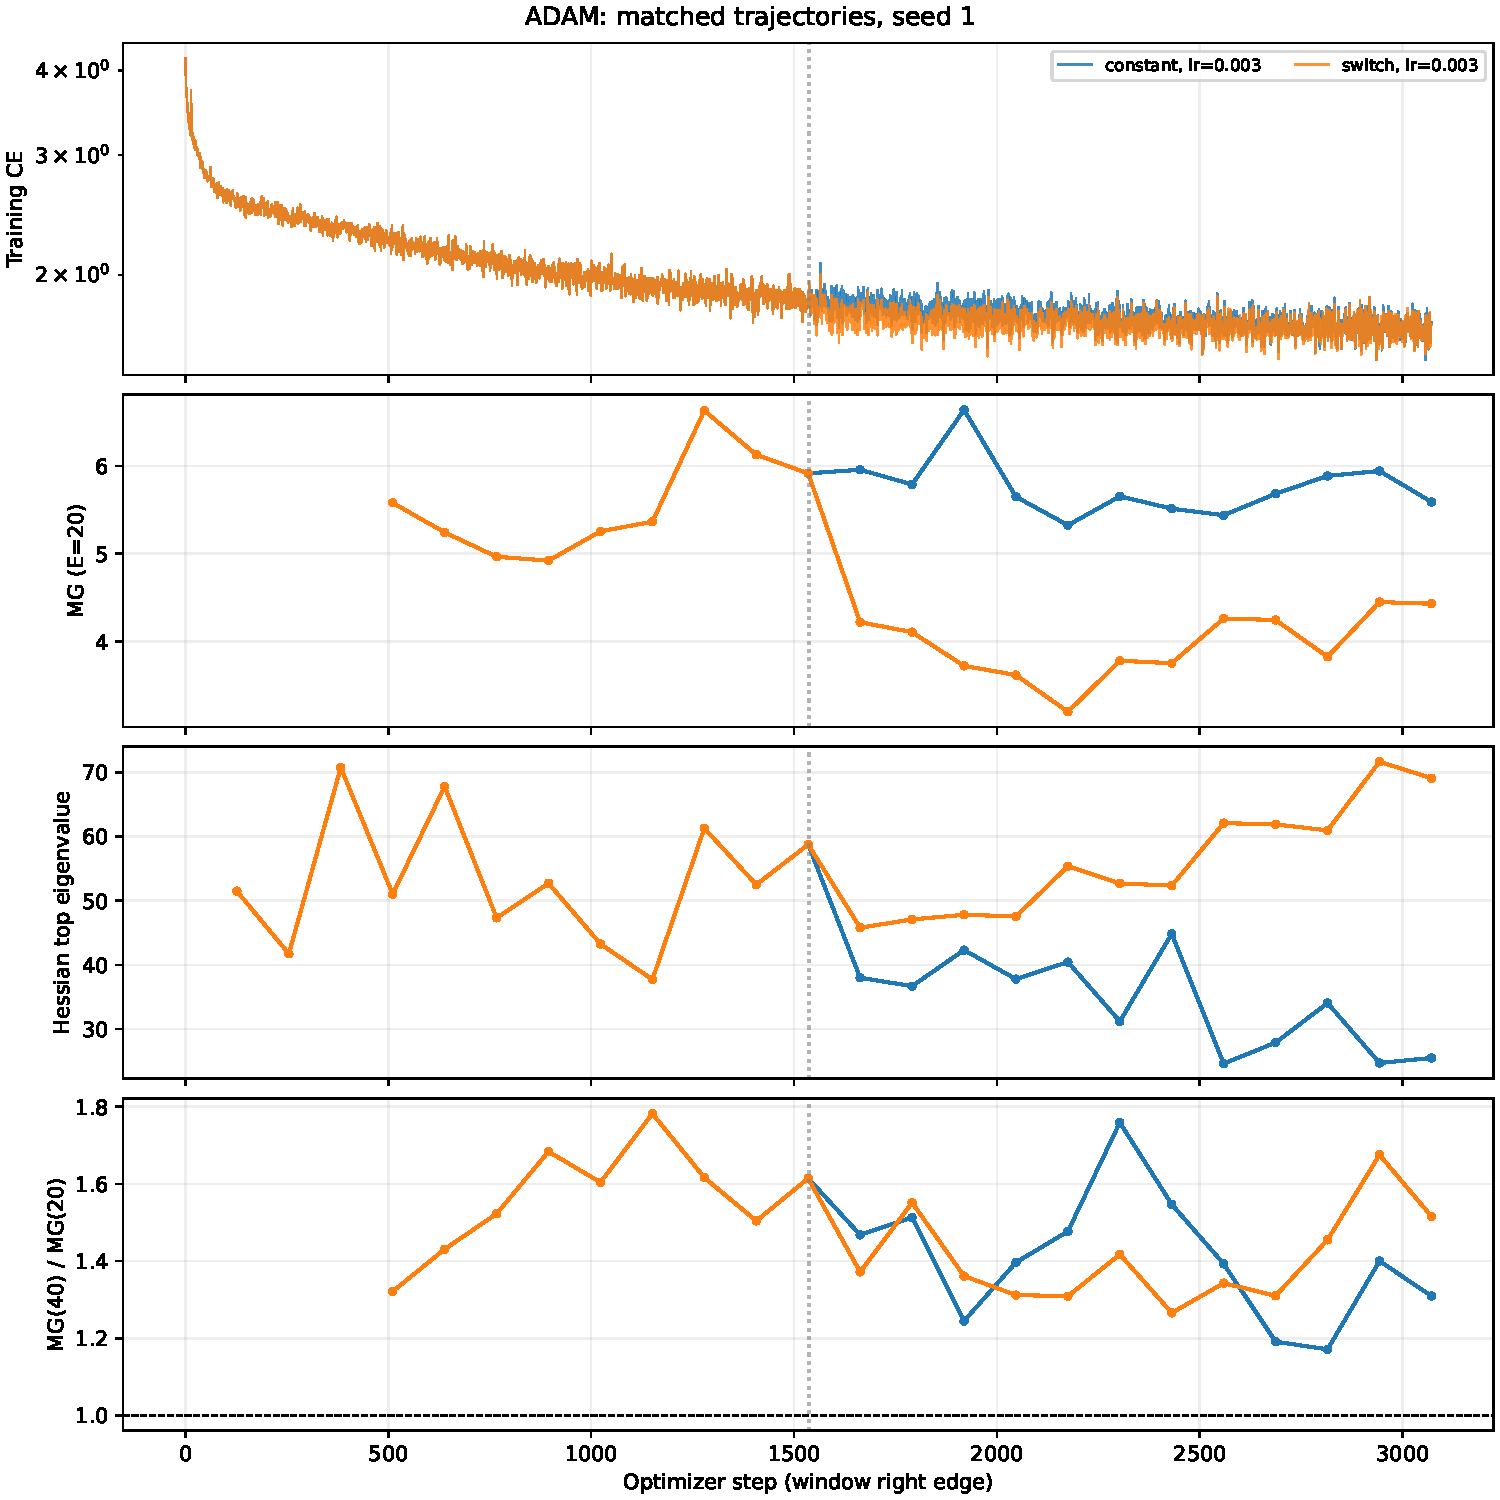
\includegraphics[width=\linewidth]{v2/adam_same_seed.pdf}
\caption{Один и тот же seed: loss, MG по probe loss, Hessian top eigenvalue и
identifiability ratio. Вертикальная линия --- смена learning rate.}
\end{figure}

\section*{4. Вычислительная стоимость}

Время измерялось на CPU при четырёх потоках, на одинаковых 21 checkpoint.

\begin{table}[h]
\centering\small
\caption{Медианная стоимость для трёх AdamW seed.}
\begin{tabular}{lrrr}
\toprule
Метод & Время, с & Hessian / метод & Комментарий \\
\midrule
Hessian top eigenvalue & 12.24 & 1.0 & Lanczos, HVP \\
MG & 0.16 & 79.7 & только scalar-log postprocessing \\
MG + validity checks & 0.37 & 33.0 & MG(40), ratio, diagnostics \\
Gradient proxy & 0.27 & 45.5 & четыре microbatch \\
Activation PR & 0.06 & 204.0 & только для этой маленькой модели \\
\bottomrule
\end{tabular}
\end{table}

Если validation probe уже логируется во время обучения, полная стоимость MG по этому
логу остаётся примерно $0.37$ с против $12.24$ с для Hessian. Если считать также
дополнительный forward на probe на каждом шаге, преимущество уменьшается примерно до
1.6 раза. Поэтому корректное сильное утверждение здесь --- ускорение по сравнению с
Hessian-анализом при наличии scalar log, а не преимущество над любой дешёвой статистикой.

\section*{5. Ограничения и решение о публикации}

Этот эксперимент пока нельзя вставлять в статью как доказательство того, что MG даёт
теоретически гарантированную active dimension в LLM training. Валидационный лог не
является явно рекуррентным, а identifiability ratio после изменения LR находится
примерно в диапазоне 1.34--1.48. Это делает интерпретацию результата exploratory:
MG надёжно фиксирует переход к более гладкой и менее изменчивой динамике probe loss,
но абсолютное значение нельзя автоматически называть числом активных компонент всей
модели.

Для публикационного эксперимента нужен Colab GPU. Следующий запуск должен использовать
модель хотя бы 10--50M параметров, 4--5 seed, несколько тысяч шагов и validation loss,
который уже считается обычным мониторингом обучения. Нужно заранее зафиксировать:
окно, задержку, Theiler exclusion, критерии валидности и способ сравнения с Hessian.
Основной claim следует формулировать как дешёвое обнаружение смены динамического режима;
claim об абсолютной dimensionality допустим только если diagnostics проходят на
контролируемом recurrent или quasi-recurrent benchmark.

\section*{6. Артефакты}

Скрипты и результаты находятся в каталоге
\texttt{research\_llm\_eos/}. Основные файлы: \texttt{run\_v2.py},
\texttt{analyze\_v2.py}, \texttt{PROTOCOL.md}, \texttt{v2/adam\_same\_seed.pdf},
\texttt{v2/effects.csv}, \texttt{v2/timing.csv}; контрольный GD находится в
\texttt{gd\_v2/}.

\end{document}
